\chapter{Elastic Search, Logstash y Kibana}\label{elastic-search-kibana-logstash}

\section{Elastic Search}\label{elastic-search}
Elasticsearch es un servidor de búsqueda basado en Lucene. Provee un motor de búsqueda de texto completo, distribuido y con capacidad de multi-tenencia con una interfaz web RESTful y con documentos JSON. Elasticsearch está desarrollado en Java y está publicado como código abierto bajo las condiciones de la licencia Apache.
Elasticsearch puede ser usado para buscar todo tipo de documentos. La búsqueda es escalable y casi en tiempo real, soportando multitenencia.Es distribuido, haciendo que los índices se puedan dividir en fragmentos y cada uno teniendo cero o más réplicas. Cada nodo alberga uno o más fragmentos, actuando como un coordinador para delegar operaciones a los fragmentos correctos. El rebalanceo y ruteo serealizan automáticamente.
Utiliza Lucene e intenta hacer todas sus funciones disponibles a través de JSON y Java API. Soporta facetado y percolación, que puede ser ùtil para notificar si nuevos documentos coinciden con consultas registradas.
Otra funcionalidad llamada gateway maneja la persistencia a largo plazo del índice por ejemplo, se puede recuperar un índice del gateway en caso de una caída del servidor. Soporta peticiones GET en tiempo real y esto lo hace válido para una solución NoSQL pero carece de transacciones distribuidas.
\section{Logstash}\label{logstash-description}

\begin{figure}
 \centering
  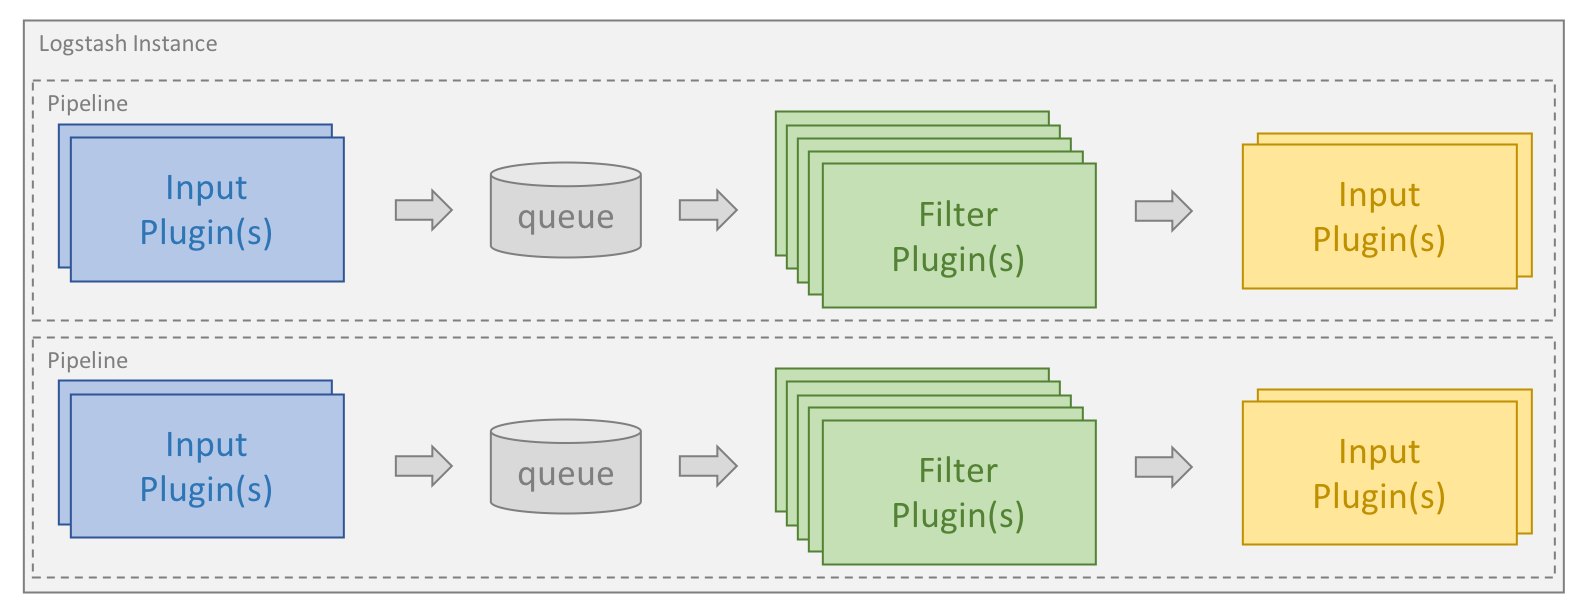
\includegraphics[width=0.5\linewidth]{./imagenes/logstash-pipeline.png}
  \caption{Logstash.}
  \label{fig:logstash}
\end{figure}

\subsection{Arquitectura de Logstash}\label{arquitectura-logtash}
Logstash es una herramienta para la administración de logs. Esta herramienta se puede utilizar para recolectar, parsear y guardar los logs para futuras búsquedas.La aplicación se encuentra basada en jRuby y requiere de Java Virtual Machine para correr. Como corre en JVM puede ser ejecutada en cualquier Sistema Operativo que corra JVM (Linux, Mac OS X, Windows).
En Logstash y con una infraestructura distribuida, cada servidor web debe ser configurado para correr Lumberjack (es opcional pero altamente recomendado para economizar recursos). Lumberjack hace un forward de los logs a un servidor corriendo Logstash con una entrada de Lumberjack. Como Lumberjack require SSL, los logs van a ser encriptados del servidor web al servidor de logs central.
Logstash is an open source, server-side data processing pipeline that ingests data from a multitude of sources simultaneously, transforms it, and then sends it to your favorite “stash.” (Ours is Elasticsearch, naturally.)	
Logstash soporta un número de entradas, códecs, filtros y salidas. Las entradas son las fuentes de datos. Los códecs esencialmente convierten un formato de entrada en un formato aceptado por Logstash, así como también transforman del formato de Logstash al formato deseado de salida. Estos son utilizados comúnmente si la fuente de datos no es una línea de texto plano. Los filtros son acciones que se utilizan para procesar en los eventos y permiten modificarlos o eliminar eventos luego de ser procesados. Finalmente, las salidas son los destinos donde los datos procesados deben ser derivados.
\section{Kibana}\label{kibana}
Kibana hace parte del grupo de aplicaciones liberadas por Elastic Search (Sharma, 2016)  para el análisis de datos a través de logs, comúnmente es conocido como “ELK Stack”, el cual refiere al uso de Elastic Search y Kibana en conjunto para la presentación y análisis de información a través de tableros de mando con estadísticas y series de tiempo.
